\documentclass{article}\usepackage[]{graphicx}\usepackage[]{color}
% maxwidth is the original width if it is less than linewidth
% otherwise use linewidth (to make sure the graphics do not exceed the margin)
\makeatletter
\def\maxwidth{ %
  \ifdim\Gin@nat@width>\linewidth
    \linewidth
  \else
    \Gin@nat@width
  \fi
}
\makeatother

\definecolor{fgcolor}{rgb}{0.345, 0.345, 0.345}
\newcommand{\hlnum}[1]{\textcolor[rgb]{0.686,0.059,0.569}{#1}}%
\newcommand{\hlstr}[1]{\textcolor[rgb]{0.192,0.494,0.8}{#1}}%
\newcommand{\hlcom}[1]{\textcolor[rgb]{0.678,0.584,0.686}{\textit{#1}}}%
\newcommand{\hlopt}[1]{\textcolor[rgb]{0,0,0}{#1}}%
\newcommand{\hlstd}[1]{\textcolor[rgb]{0.345,0.345,0.345}{#1}}%
\newcommand{\hlkwa}[1]{\textcolor[rgb]{0.161,0.373,0.58}{\textbf{#1}}}%
\newcommand{\hlkwb}[1]{\textcolor[rgb]{0.69,0.353,0.396}{#1}}%
\newcommand{\hlkwc}[1]{\textcolor[rgb]{0.333,0.667,0.333}{#1}}%
\newcommand{\hlkwd}[1]{\textcolor[rgb]{0.737,0.353,0.396}{\textbf{#1}}}%
\let\hlipl\hlkwb

\usepackage{framed}
\makeatletter
\newenvironment{kframe}{%
 \def\at@end@of@kframe{}%
 \ifinner\ifhmode%
  \def\at@end@of@kframe{\end{minipage}}%
  \begin{minipage}{\columnwidth}%
 \fi\fi%
 \def\FrameCommand##1{\hskip\@totalleftmargin \hskip-\fboxsep
 \colorbox{shadecolor}{##1}\hskip-\fboxsep
     % There is no \\@totalrightmargin, so:
     \hskip-\linewidth \hskip-\@totalleftmargin \hskip\columnwidth}%
 \MakeFramed {\advance\hsize-\width
   \@totalleftmargin\z@ \linewidth\hsize
   \@setminipage}}%
 {\par\unskip\endMakeFramed%
 \at@end@of@kframe}
\makeatother

\definecolor{shadecolor}{rgb}{.97, .97, .97}
\definecolor{messagecolor}{rgb}{0, 0, 0}
\definecolor{warningcolor}{rgb}{1, 0, 1}
\definecolor{errorcolor}{rgb}{1, 0, 0}
\newenvironment{knitrout}{}{} % an empty environment to be redefined in TeX

\usepackage{alltt}

% set font encoding for PDFLaTeX, XeLaTeX, or LuaTeX
\usepackage{ifxetex,ifluatex}
\if\ifxetex T\else\ifluatex T\else F\fi\fi T%
  \usepackage{fontspec}
\else
  \usepackage[T1]{fontenc}
  \usepackage[utf8]{inputenc}
  \usepackage{lmodern}
\fi

\usepackage{bookmark} %Para bookmark del indice
\usepackage{hyperref} %Uso de vinculos
\usepackage{afterpage} %Agregar paginas en blanco
\usepackage{amsfonts} %Formulas matematicas
\usepackage{amsmath} %Alinear ecuaciones y similar
\usepackage{sagetex} %Hacer calculos
\usepackage{fullpage} %Trabajar con menos margenes de pagina
\usepackage{xcolor}  %Usar colores
\usepackage{graphicx} %Agregar imagenes
\usepackage{apacite} %Trabajar bibliografias APA
\usepackage{venndiagram} %Agregar diagramas de Venn
\usepackage{pdfpages} %Incluir pdf externos
\usepackage{natbib} %Agregar Bibliografias
\usepackage[spanish]{babel} %Configurar el idioma
\usepackage[shortlabels]{enumitem} %Para enumerar con letras
\usepackage{float}
\IfFileExists{upquote.sty}{\usepackage{upquote}}{}
\begin{document}

\begin{titlepage}
\centering
{
\includegraphics[width=0.2\textwidth]{logoUCR}\par}
\vspace{1cm}
{\bfseries\LARGE Universidad de Costa Rica \par}
\vspace{1cm}
{\scshape\Large Facultad de Ingenier\'ia \par}
{\scshape\Large Escuela de Ciencias de la Computaci\'on e Inform\'atica \par}
\vspace{1cm}
{\scshape\Large CI0115 – PROBABILIDAD Y ESTADÍSTICA \par}
{\scshape\Large Profesora Kryscia Ram\'irez \par}
\vspace{1cm}
{\scshape\Huge Tarea 02 \par}
\vspace{1cm}
{\Large Estudiante: \par}
{\Large Emmanuel Sol\'is \par}
{\Large \textit{\color{blue}emmanuel.solisp@icloud.com} \par}
\vspace{2cm}
{\Large 23 de septiembre de 2020 \par}
\end{titlepage}

\newpage
\tableofcontents

\newpage
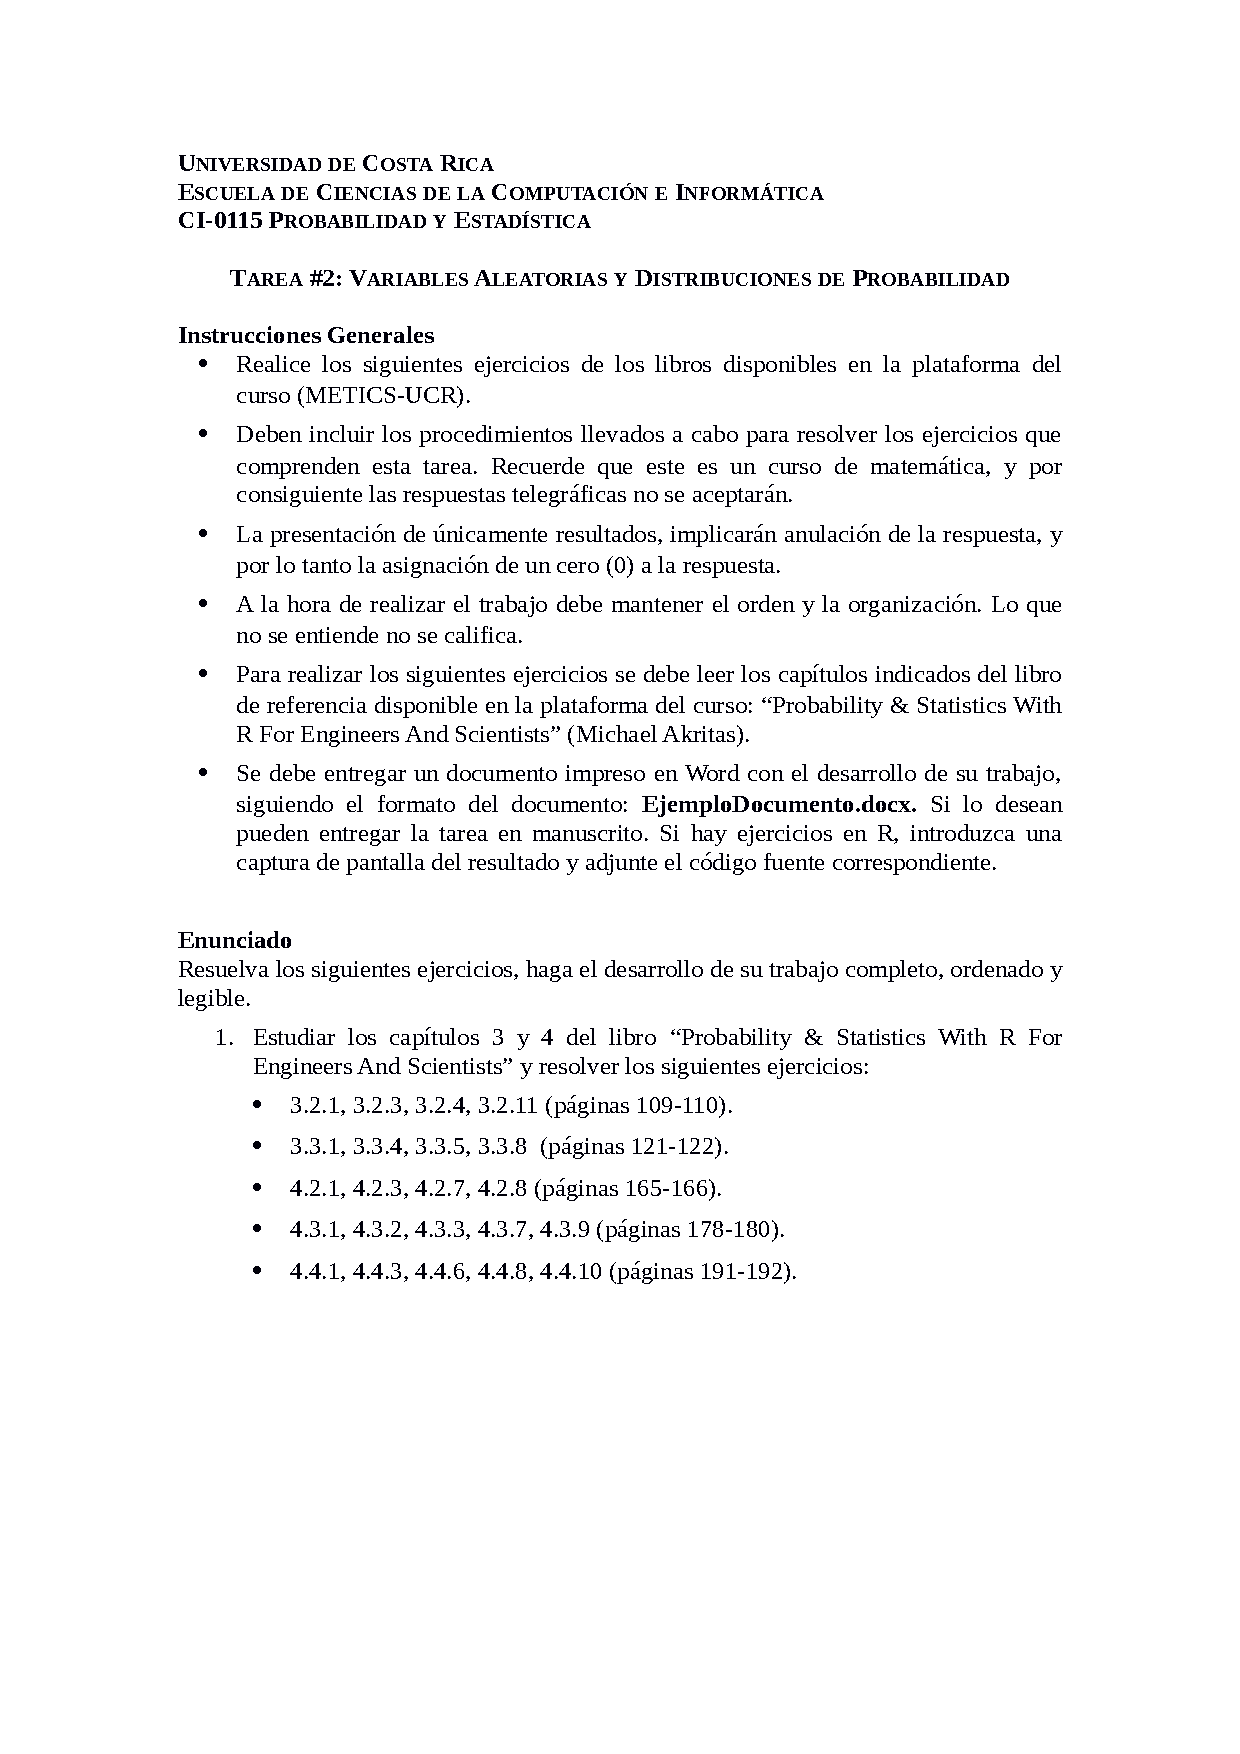
\includepdf[pages={-}]{Enunciado.pdf}

%---------------- SageSilent -------------------------
\begin{sagesilent}
#Para la funcion del ejercicio 4.2.7 -> Hecho por Emmanuel.
k = var('k')
y = var('y')
fx = k*x*y^(2)
fxdx = integrate(fx, x, 0, 2)
fxdy = integrate(fxdx, y, 2, 3)
valorK = solve(fxdy==1, k)
\end{sagesilent}
%---------------- Solucion de ejercicios -------------------------
%NOTA: Si van a usar referencias hacer la cita con:
%\cite{Wal07} si es el libro Probability and ...
%\cite{Hor09} si es el libro del ejercicio en R
%NOTA 2: Usar \subsection{} 

\section{Solución de ejercicios}

\subsection{Ejercicio 3.2.1}
\begin{enumerate}[a)]
    \item Verifique que $p_{1}(x)$ y $p_{2}(x)$ son funciones de masa de probabilidad legítimas.

\textbf{Respuesta:} Una de las propiedades que son necesarias verificar es que la suma sea igual a 1 y que sus valores estén entre 0 y 1. Entonces:
\[p_{1}(x) = 0.3+0.3+0.5-0.1 = 1\]
\[p_{2}(x) = 0.1+0.4+0.4+0.1 = 1\]
Es posible observar que se cumple la propiedad de que la suma sea igual a 1, pero en el caso del $p_{1}(x)$ tiene un valor negativo por lo tanto no es función de masa, en cambio $p_{2}(x)$ si es función de masa.

    \item Calcule el valor de $k$ para que $p(x)$ sea una función de masa de probabilidad.

\textbf{Respuesta:} Se resuelve la siguiente ecuación:
\begin{align*}
    0.2k+0.3k+0.4k+0.2k &= 1\\
    1.1k &= 1\\
    k &= \frac{1}{1.1} = \frac{1}{\frac{11}{10}} = \frac{11}{10}
\end{align*}
Por lo tanto para que se cumpla que $p(x)$ sea una función de masa de probabilidad $k$ debe ser $k = \frac{10}{11}$.
\end{enumerate}


\subsection{Ejercicio 3.2.3}

\begin{enumerate}
    \item Grafique la CDF.

\textit{Solución: }

Con el siguiente código logramos plasmar el código de CDF.

\begin{knitrout}
\definecolor{shadecolor}{rgb}{0.969, 0.969, 0.969}\color{fgcolor}\begin{kframe}
\begin{alltt}
  \hlstd{datosCDF} \hlkwb{=} \hlkwd{read.table}\hlstd{(}\hlstr{"CDFdatos.txt"}\hlstd{,} \hlkwc{sep} \hlstd{=} \hlstr{","}\hlstd{,} \hlkwc{header} \hlstd{= T)}
 \hlkwd{plot}\hlstd{(}\hlkwd{ecdf}\hlstd{(datosCDF} \hlopt{$} \hlstd{funcionCDF),} \hlkwc{ylab}\hlstd{=}\hlstr{"F(y)"}\hlstd{,} \hlkwc{xlab}\hlstd{=}\hlstr{"y"}\hlstd{,} \hlkwc{main} \hlstd{=} \hlstr{"Función De CDF"}\hlstd{,} \hlkwc{cex}\hlstd{=}\hlnum{0}\hlstd{)}
\end{alltt}
\end{kframe}

{\centering 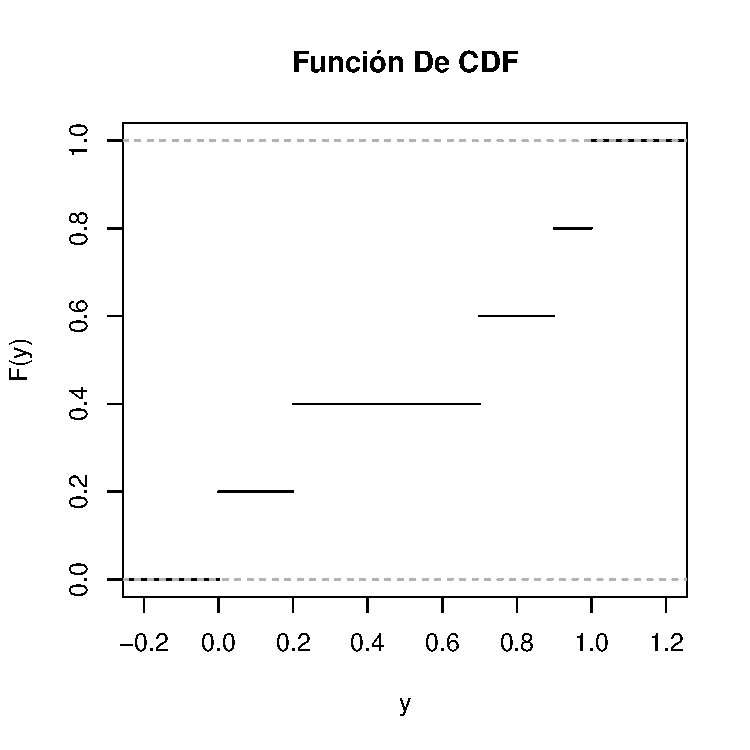
\includegraphics[width=0.5\linewidth]{figure/unnamed-chunk-1-1} 

}



\end{knitrout}
 \item Encuentre la probabilidad de que el costo de retrasos será de al menos $ \$200,00.$
 
 \textit{Solución :}
 
Podemos observar que para el costo sea de al menos de $\$200$, es de $3 \leq y$ y $1\leq y < 2$.

Por lo tanto: 
\begin{center}
$P(Y < y)= F(Y)= 1 - 0.7 = 0.3 $
\end{center}

Como resultado tenemos una probabilidad $0.3$ de que el costo de los retrasos sea de al menos $ \$200 $

    \item Encuentre la función de masa de probabilidad de Y
    
Sea X el número de piezas completadas por su plazo y sea Y el costo, en cientos de dólares, incurrido a la planta de fabricación de metal, según el enunciado.

Entonces tenemos que:


\begin{center}
$f(x)=P(Y=x)= \frac{\binom{3}{x} }{6}=$ Para 0,1,2,3.
\end{center}

\begin{center}
\begin{table}[h]
\centering
\def\arraystretch{1.5}
\begin{tabular}{c|c c c c }
y & 0 & 1 & 2 & 3\\ \hline
h(y) & $0.2$ & $0.5$ & $0.2$ & $0.1$
\end{tabular}
\end{table}
\end{center}
\end{enumerate}

\subsection{Ejercicio 3.2.4} Hallar la \textit{funci\'on de masa de probabilidad} y la \textit{funci\'on de distribuci\'on acumulada}.
\begin{enumerate}
\item Hallar la funci\'on de masa de probabilidad.\\
\textbf{Soluci\'on:} dado que se extraen solo $3$ de los $10$ art\'iculos, $x$ solo puede tomar los valores $x=0,1,2,3$. Por lo tanto calculamos las probabilidades para cada valor de $x$:
\begin{center}
$f(0) = \frac{\binom{4}{0}\cdot \binom{6}{3}}{\binom{10}{3}} = \sage{(binomial(4, 0)*binomial(6,3))/binomial(10,3)}, f(1) = \frac{\binom{4}{1}\cdot \binom{6}{2}}{\binom{10}{3}} = \sage{(binomial(4, 1)*binomial(6,2))/binomial(10,3)}, f(2) = \frac{\binom{4}{2}\cdot \binom{6}{1}}{\binom{10}{3}} = \sage{(binomial(4, 2)*binomial(6,1))/binomial(10,3)}, f(3) = \frac{\binom{4}{3}\cdot \binom{6}{0}}{\binom{10}{3}} = \sage{(binomial(4, 3)*binomial(6,0))/binomial(10,3)}$

\begin{table}[h]
\centering
\def\arraystretch{1.5}
\begin{tabular}{c|c c c c }
x & 0 & 1 & 2 & 3\\ \hline
f(x) & $\frac{1}{6}$ & $\frac{1}{2}$ & $\frac{3}{10}$ & $\frac{1}{30}$
\end{tabular}
\end{table}
\end{center}

\item Hallar la funci\'on de distribuci\'on acumulativa.\\
\textbf{Soluci\'on:} hallar esta funci\'on es m\'as sencillo dado que solo debemos para cada probabilidad de $x$ sumarle la probabilidad desde $x=0$ el $x$ que nos piden:
\begin{itemize}
\item $f(0) = \frac{1}{6}$
\item $f(1) = \frac{1}{6} + \frac{1}{2} = \sage{(1/6)+(1/2)}$
\item $f(2) = \frac{1}{6} + \frac{1}{2} + \frac{3}{10} = \sage{(1/6)+(1/2)+(3/10)}$
\item $f(3) = \frac{1}{6} + \frac{1}{2} + \frac{3}{10} +\frac{1}{30} = \sage{(1/6)+(1/2)+(3/10) + (1/30)}$
\end{itemize}
\end{enumerate}

\subsection{Ejercicio 3.2.11}
Se nos pide utilizar varios comandos para generar histogramas de varias muestras, de tamaños 100, 1000, 10000 y 100000 para luego sobreponer la función de densidad de probabilidad uniforme sobre el histograma, de esta manera en R: 


\begin{knitrout}
\definecolor{shadecolor}{rgb}{0.969, 0.969, 0.969}\color{fgcolor}\begin{kframe}
\begin{alltt}
\hlkwd{set.seed}\hlstd{(}\hlnum{111}\hlstd{)}
\hlkwd{hist}\hlstd{(}\hlkwd{runif}\hlstd{(}\hlnum{100}\hlstd{),} \hlkwc{freq}\hlstd{=F)}
\hlkwd{curve}\hlstd{(dunif,} \hlnum{0}\hlstd{,} \hlnum{1}\hlstd{,} \hlkwc{add}\hlstd{=T)}
\end{alltt}
\end{kframe}
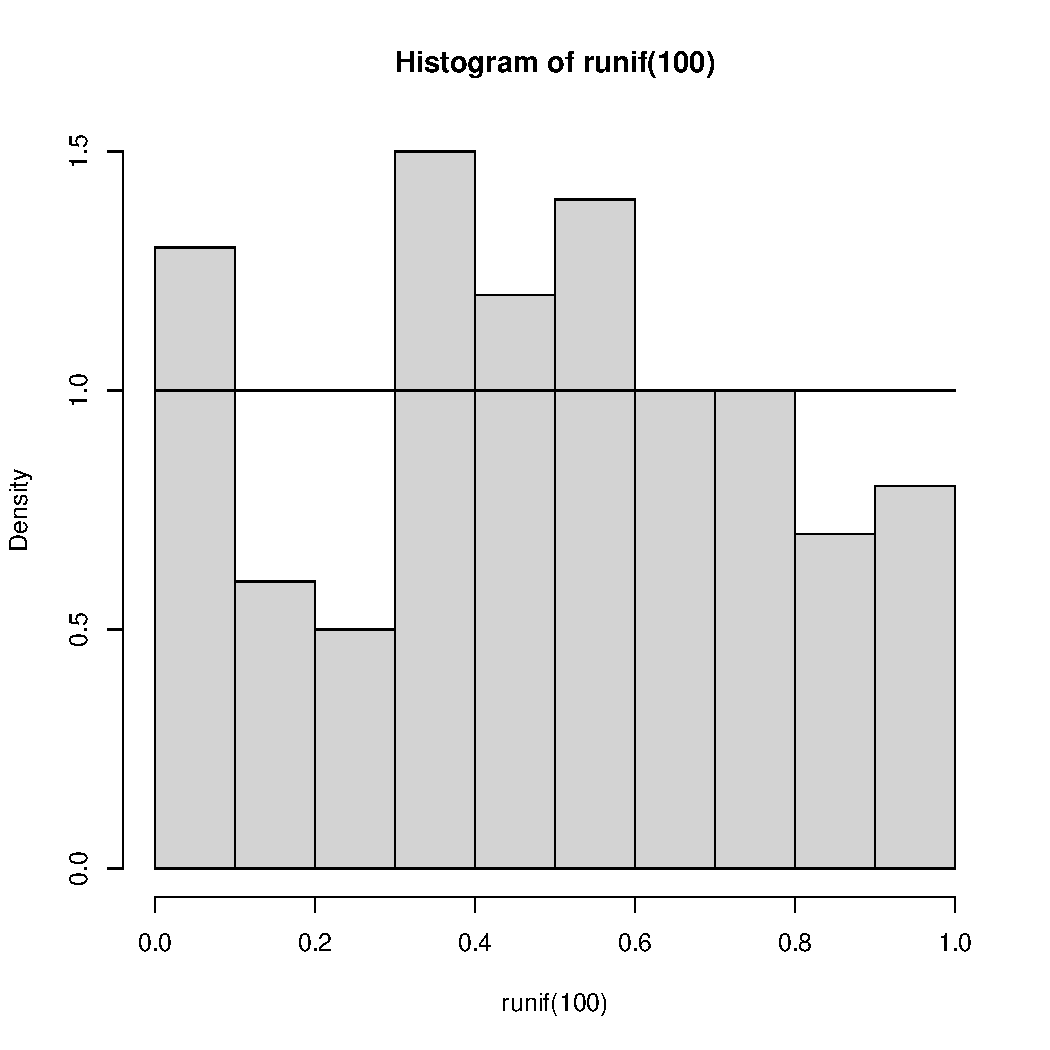
\includegraphics[width=\maxwidth]{figure/unnamed-chunk-2-1} 

\end{knitrout}


Para luego analizar lo siguiente:
\begin{itemize}
\item ¿El histograma provee una aproximación razonable a la función de densidad de probabilidad uniforme con una muestra de tamaño 100?

\textbf{Respuesta:} Es una aproximación aceptable, pero no se aproxima lo suficiente, hay mucha variedad en la muestra.
\item 
¿Para que tamaño de muestras podría decir que el histograma provee una aproximación razonable a la función de densidad de probabilidad?

\textbf{Respuesta:} Con valores superiores a 10000, ya se obtiene una aproximación muy razonable, y entre mas valores se inserten, mas se aproximara.

\end{itemize}

\subsection{Ejercicio 3.3.1}
Una muestra aleatoria simple de 3 items es seleccionado de un cargamento de 20 items de los cuales 4 están defectuosos. Sea X el número de items defectuosos en la muestra.
\begin{enumerate}[(a)]
    \item Encuentre la función de masa de probabilidad de X.
Se saca la combinación total de sacar 3 items, lo cual corresponde a $C(20,3) = 1140$. Y se calculan cada una de las probabilidades:
\begin{align*}
f(0) &= \frac{{4 \choose 0} {16 \choose 3}}{{20 \choose 3}} = \frac{28}{57}\\
f(1) &= \frac{{4 \choose 1} {16 \choose 2}}{{20 \choose 3}} = \frac{8}{19}\\
f(2) &= \frac{{4 \choose 2} {16 \choose 1}}{{20 \choose 3}} = \frac{8}{95}\\
f(3) &= \frac{{4 \choose 3} {16 \choose 0}}{{20 \choose 3}} = \frac{1}{285}\\
\end{align*}
\begin{table}[H]
\centering
\def\arraystretch{1.5}
\begin{tabular}{c|c c c c }
x    & 0     & 1    & 2    & 3     \\ \hline
f(x) & $\frac{28}{75}$ & $\frac{8}{19}$ & $\frac{8}{95}$ & $\frac{1}{285}$
\end{tabular}
\end{table}

    \item Encuentre la media y la varianza de X.
    
Para la media la fórmula corresponde a:
\[\mu_{x} = \sum_{x}xf(x)\]
Entonces:
\begin{align*}
    \sum_{x}xf(x) &= 0*\frac{28}{75}+1*\frac{8}{19}+2*\frac{8}{95}+3*\frac{1}{285}\\
    &= 0 + \frac{8}{19} + \frac{16}{95} + \frac{3}{285}\\
    &= \frac{3}{5}
\end{align*}
Y para la varianza corresponde a:
\[\sigma^{2} = E[(x-\mu)^{2}] = \sum_{x}(x-\mu)^{2}f(x)\]
Por lo tanto:
\begin{align*}
    \sigma^{2} &= \left(0-\frac{3}{5}\right)^{2}*\frac{28}{57}+\left(1-\frac{3}{5}\right)^{2}*\frac{8}{19}+\left(2-\frac{3}{5}\right)^{2}*\frac{8}{95}+\left(3-\frac{3}{5}\right)^{2}*\frac{1}{285}\\
    &= \frac{84}{475}+\frac{32}{475}+\frac{392}{2375}+\frac{48}{2375}\\
    &= \frac{204}{475} \approx 0,4295
\end{align*}
\end{enumerate}

\subsection{Ejercicio 3.3.4}
\begin{enumerate}
    \item Compute la esperanza y la varianza de $X$.
    
    \textit{Solución: }
    
Utilizamos el siguiente codigo en R:

\begin{knitrout}
\definecolor{shadecolor}{rgb}{0.969, 0.969, 0.969}\color{fgcolor}\begin{kframe}
\begin{alltt}
\hlstd{x}\hlkwb{=} \hlkwd{c}\hlstd{(}\hlnum{0}\hlstd{,}\hlnum{1}\hlstd{,}\hlnum{2}\hlstd{,}\hlnum{3}\hlstd{,}\hlnum{4}\hlstd{,}\hlnum{5}\hlstd{)}
\hlstd{p}\hlkwb{=} \hlkwd{c}\hlstd{(}\hlnum{.05}\hlstd{,}\hlnum{.10}\hlstd{,}\hlnum{.15}\hlstd{,}\hlnum{.25}\hlstd{,}\hlnum{.35}\hlstd{,}\hlnum{.10}\hlstd{)}

\hlstd{E}\hlkwb{<-}\hlkwd{sum}\hlstd{(x}\hlopt{*}\hlstd{p)}
\hlstd{E}
\end{alltt}
\begin{verbatim}
## [1] 3.05
\end{verbatim}
\begin{alltt}
\hlkwd{sum}\hlstd{((x}\hlopt{-}\hlstd{E)}\hlopt{*}\hlstd{(x}\hlopt{-}\hlstd{E)}\hlopt{*}\hlstd{p)}
\end{alltt}
\begin{verbatim}
## [1] 1.7475
\end{verbatim}
\end{kframe}
\end{knitrout}
Como resultado tenemos una $E(X)= 3.05$ y una $Var(X)= 1.7475$

\item Por cada pieza completa antes de su plazo, la planta recibe un bonus de $\$15000 $. Encuentre la esperanza y la varianza del bonus total.

\textit{Solución:}

Utilizaremos el siguiente código en R.
\begin{knitrout}
\definecolor{shadecolor}{rgb}{0.969, 0.969, 0.969}\color{fgcolor}\begin{kframe}
\begin{alltt}
\hlstd{x}\hlkwb{=} \hlkwd{c}\hlstd{(}\hlnum{0}\hlstd{,}\hlnum{1}\hlstd{,}\hlnum{2}\hlstd{,}\hlnum{3}\hlstd{,}\hlnum{4}\hlstd{,}\hlnum{5}\hlstd{)}
\hlstd{p}\hlkwb{=} \hlkwd{c}\hlstd{(}\hlnum{.05}\hlstd{,}\hlnum{.10}\hlstd{,}\hlnum{.15}\hlstd{,}\hlnum{.25}\hlstd{,}\hlnum{.35}\hlstd{,}\hlnum{.10}\hlstd{)}

\hlstd{E} \hlkwb{<-} \hlkwd{sum}\hlstd{((x}\hlopt{*}\hlnum{15000}\hlstd{)}\hlopt{*}\hlstd{p)}

\hlkwd{sum}\hlstd{((x}\hlopt{*}\hlnum{15000}\hlopt{-}\hlstd{E)}\hlopt{*}\hlstd{(x}\hlopt{*}\hlnum{15000}\hlopt{-}\hlstd{E)}\hlopt{*}\hlstd{p)}
\end{alltt}
\begin{verbatim}
## [1] 393187500
\end{verbatim}
\begin{alltt}
\hlstd{E}
\end{alltt}
\begin{verbatim}
## [1] 45750
\end{verbatim}
\end{kframe}
\end{knitrout}

Como resultado tenemos una $E(15.000X)= 45750$ y una $Var(15.000X)= 393187500$

\end{enumerate}

\subsection{Ejercicio 3.3.5} Halle, usando \textit{R}, la \textit{esperanza matem\'atica} y la \textit{varianza} de la funci\'on:
\begin{center}
$f(x) = \begin{cases} \frac{1}{100}x \cdot e^{-x/10} ,x > 0 \\ 0, x\leq 0 \end{cases}$
\end{center}
\textbf{Soluci\'on:}
\begin{enumerate}
\item Hallar la esperanza matem\'atica $E(X)$.
\begin{knitrout}
\definecolor{shadecolor}{rgb}{0.969, 0.969, 0.969}\color{fgcolor}\begin{kframe}
\begin{alltt}
\hlstd{e} \hlkwb{<-} \hlkwd{sum}\hlstd{(}\hlnum{1}\hlopt{/}\hlkwd{factorial}\hlstd{(}\hlnum{0}\hlopt{:}\hlnum{100}\hlstd{))} \hlcom{#Calculo el valor de Euler.}
\hlstd{fun} \hlkwb{<-} \hlkwa{function}\hlstd{(}\hlkwc{x}\hlstd{) ((}\hlnum{1}\hlopt{/}\hlnum{1000}\hlstd{)}\hlopt{*}\hlstd{x}\hlopt{*}\hlstd{e}\hlopt{^}\hlstd{(}\hlopt{-}\hlstd{x}\hlopt{/}\hlnum{10}\hlstd{))}\hlopt{*}\hlstd{x} \hlcom{#Calculo de la integral x*f(x)}
\hlstd{esperanzaMatematica} \hlkwb{<-} \hlkwd{integrate}\hlstd{(fun,} \hlnum{0}\hlstd{,} \hlnum{Inf}\hlstd{)}
\hlstd{esperanzaMatematica}
\end{alltt}
\begin{verbatim}
## 2 with absolute error < 8.1e-08
\end{verbatim}
\end{kframe}
\end{knitrout}
Por lo tanto $E(X)=2$. El valor m\'as esperado de duraci\'on es $2$.

\item Hallar la varianza $\sigma^{2}$.
\begin{knitrout}
\definecolor{shadecolor}{rgb}{0.969, 0.969, 0.969}\color{fgcolor}\begin{kframe}
\begin{alltt}
\hlstd{fun} \hlkwb{<-} \hlkwa{function}\hlstd{(}\hlkwc{x}\hlstd{) ((}\hlnum{1}\hlopt{/}\hlnum{1000}\hlstd{)}\hlopt{*}\hlstd{x}\hlopt{*}\hlstd{e}\hlopt{^}\hlstd{(}\hlopt{-}\hlstd{x}\hlopt{/}\hlnum{10}\hlstd{))}\hlopt{*}\hlstd{x}\hlopt{^}\hlstd{(}\hlnum{2}\hlstd{)} \hlcom{#Calculo de la integral x^2*f(x)}
\hlstd{u} \hlkwb{<-} \hlnum{2}\hlopt{^}\hlnum{2}
\hlstd{varianza} \hlkwb{<-} \hlkwd{integrate}\hlstd{(fun,} \hlnum{0}\hlstd{,} \hlnum{Inf}\hlstd{)} \hlcom{#Sabemos que varianza = E(X^2) - u^2}
\hlstd{varianza}
\end{alltt}
\begin{verbatim}
## 60 with absolute error < 7e-05
\end{verbatim}
\begin{alltt}
\hlstd{varianza} \hlkwb{<-} \hlnum{60}\hlopt{-}\hlstd{(}\hlnum{2}\hlopt{^}\hlnum{2}\hlstd{)} \hlcom{#Hago la resta y me da la varianza.}
\hlstd{varianza}
\end{alltt}
\begin{verbatim}
## [1] 56
\end{verbatim}
\end{kframe}
\end{knitrout}
Por lo tanto tenemos que dado el \textit{Teorema} $4.2$ \cite[~p\'ag. 121]{Wal07}, la varianza es $\sigma^{2}=56$.
\end{enumerate}

\subsection{Ejercicio 3.3.8}

La cantidad de tiempo X, en horas, que un libro de referencia de estadística en una reserva de 2 horas en la librería de ingeniería es cogido prestado por un estudiante aleatorio, tiene una función de densidad de probabilidad de:
$$f(x,y) \begin{cases} \frac{1}{log(4)}\cdot \frac{1}{1+x}, 0 \leq x \leq 3
 \\ 0, otherwise\end{cases} $$
 

Por los libros devueltos después de 2 horas, los estudiantes son multados por 2 dolares mas 6 centavos multiplicados por la cantidad de minutos después de las 2 horas.
\begin{itemize}
\item Si Y = 60X es la cantidad de tiempo en minutos que el libro ha sido retirado. Encuentre la función de densidad de probabilidad de Y.

\textbf{Respuesta:}

\[=\int_{0}^{\frac{Y}{60}}\frac{1}{log(4)}\cdot \frac{1}{\frac{1}{1+\frac{y}{60}}}dy=\frac{1}{log(4)}\int_{1}^{1+x}\frac{1}{\frac{y}{60}}=\frac{log(1+\frac{1}{60})}{log(4)}\]

\item Si V es la cantidad de multa en centavos, que un estudiante pagara, encuentre E(V) y $\sigma ^{2}_{V}$

\textbf{Respuesta:}

\[E(V) = \int_{0}^{1}x(\frac{1}{log(4)}\cdot \frac{1}{1+x})dx = \frac{-4ln(2)+4}{8ln(2)}\]

\[E(V^{2}) = \int_{0}^{1}x^{2}(\frac{1}{log(4)}\cdot \frac{1}{1+x})dx = \frac{-\pi +4}{8ln(2)}\]

\[\sigma ^{2}_{v} = \frac{-\pi +4}{8ln(2)}-(\frac{-4ln(2)+4}{8ln(2)})^{2} = 0.10581\]





\end{itemize}


 
\subsection{Ejercicio 4.2.1}
Sea X el número de compras diarias de un objeto de lujo de un lugar de fábrica outlet y Y el número diario de compras hechas en línea. Sea los valores 1,2 y 3 el número de compras menores a cinco, al menos cinco pero menos que 15, y 15 o más, respectivamente. Suponga que la función de masas de probabilidad conjunta de X y Y es:
\begin{table}[h]
\centering
\begin{tabular}{cc|ccc}
                       &        &                           & y                         &      \\ \cline{3-5} 
                       & p(x,y) & \multicolumn{1}{c|}{1}    & \multicolumn{1}{c|}{2}    & 3    \\ \hline
\multicolumn{1}{c|}{}  & 1      & \multicolumn{1}{c|}{0.09} & \multicolumn{1}{c|}{0.12} & 0.13 \\ \hline
\multicolumn{1}{c|}{x} & 2      & \multicolumn{1}{c|}{0.12} & \multicolumn{1}{c|}{0.11} & 0.11 \\ \hline
\multicolumn{1}{c|}{}  & 3      & \multicolumn{1}{c|}{0.13} & \multicolumn{1}{c|}{0.10} & 0.09
\end{tabular}
\end{table}
\begin{enumerate}[(a)]
    \item Encuentre la probabilidad de cada uno de los eventos:
    \begin{itemize}
        \item $(X>1,Y>2)$: corresponden los valores 0.11 y 0.09 entonces $P(X>1,Y>2) = 0.11+0.09 = 0.2$
        \item $(X>1 \text{ or } Y>2)$: corresponden los valores 0.12, 0.11, 0.11, 0.13, 0.10 y 0.09 entonces: $P(X>1 \text{ or } Y>2) = 0.12+0.11+0.11+0.13+0.10+0.09 = 0.66$
        \item $(X > 2,Y > 2)$: corresponden al valor de 0.09 entonces $P(X > 2,Y > 2) = 0.09$
    \end{itemize}
    
    \item Encuentre la función de masa de probabilidad marginal de X y de Y.
    
    \textbf{Respuesta:} Se puede calcular realizando la suma de cada una de las columnas y filas del cuadro de función de masas de probabilidad conjunta, entonces para X corresponde a:
    \begin{align*}
        P(X=1) &= 0.09+0.12+0.13 = 0.34\\
        P(X=2) &= 0.12+0.11+0.11 = 0.34\\
        P(X=3) &= 0.13+0.10+0.09 = 0.32
    \end{align*}
    Para Y corresponde a:
    \begin{align*}
        P(Y=1) &= 0.09+0.12+0.13 = 0.34\\
        P(Y=2) &= 0.12+0.11+0.10 = 0.33\\
        P(Y=3) &= 0.13+0.11+0.09 = 0.33
    \end{align*}
    \end{enumerate}

\subsection{Ejercicio 4.2.3}
\begin{enumerate}
    \item Encontrar la probabilidad de $(X \leq 10, Y\leq 2)$ y $(X\leq 10, Y=2)$
    
\textit{Solución :}


\begin{center}

Probabilidad de: $ P(X \leq 10, Y \leq  2)$

$= P(X = 8, Y = 1.50) + P(X = 8, Y = 2) + P(X = 10, Y=1.50) +P(X=10, Y=2)$

$= 0.3 + 0.12 + 0.15 + 0.135$

$= 0.705 $ 


Probabilidad de:   $P(X\leq 10, Y = 2)$

$= P(X\leq 10, Y = 2)= P(X = 8, Y = 2)+P(X = 10,Y = 2)$

$= 0.12 + 0.135 $

$= 0.255$
\end{center}

\item Calcule los PMF marginales de X e Y.

\textit{Solución:}

Marginales de X:

\begin{center}
$PX(8) = 0.3 + 0.12 + 0 = \textbf{0.42}$

$PX(10) = 0.15 + 0.135 + 0.02 = \textbf{0.31} $

$PX(12) = 0.03 + 0.15 + 0.09 = \textbf{0.27}$
\end{center}

Marginales de Y:


\begin{center}
$PY(1.5)= 0.3 + 0.15 + 0.03 = \textbf{0.48}$

$PY(2) = 0.12 + 0.135 + 0.15 = \textbf{0.405}$

$PY(2.5) =0  + 0.025 + 0.09 = \textbf{0.115}$
\end{center}

\item Dado que un cliente ha dejado una propina de  $\$2.00 $, encuentre la probabilidad de que el cliente haya pedido una comida de  $ \$10.00$ o menos.

\textit{Solución :}

Para resolver el ejercicio necesitamos encontrar $f(x|y)$, donde $y = 2$. Primero, utilizaremos la  distribución condicional de X, dado que
Y = 2, y la utilizaremos para determinar $P(X \leq 10|Y = 2)$.

Siendo así tenemos:

\begin{center}
$h(2)= \sum_{x=0}^{2}f(x,2)=0.2+ 0.135 + 0.15 = 0.405 $
\end{center}

Utilizando la distribución de probabilidad condicional para $X=10, X=8, Y=2$:

\begin{center}
$f(x|2)= \frac{f(8,2)}{h(2)}= \frac{0.12}{0.405}=\frac{8}{27}$

$f(x|2)= \frac{f(10,2)}{h(2)}= \frac{0.135}{0.405}=\frac{1}{3}$

$f(x|2)= \frac{8}{27} + \frac{1}{3}= \textbf{0.6296}$
\end{center}

Por lo tanto la probabilidad de que un cliente haya pedido una comida de $\$10$ o menos, dado una propina de $\$2$ es de \textbf{0.6296}.


\end{enumerate}

\subsection{Ejercicio 4.2.7} Tenemos $f(x,y) \begin{cases} kxy^{2}, 0\leq x \leq 2, x\leq y \leq 3 \\ 0, elsewhere \end{cases} $.
\begin{enumerate}
\item Halle la constante $k$: para hallar este resultado tenemos que es seguro que el \'area bajo la curva debe ser $1$ por lo tanto tenemos:\\
$$1 = \int_{2}^{3} \int_{0}^{2} \sage{fx} dxdy$$\\
$$1 = \int_{2}^{3} \sage{integrate(fx, x)} \Big{|}_{0}^{2}dy = \sage{fxdx}$$\\
$$1 = \sage{fxdx} \Big{|}_{2}^{3} = \sage{fxdy}$$\\
$$\sage{valorK}$$\\
Por lo tanto tenemos que el valor $k=\sage{valorK}$.

\item Halle la funci\'on de distribuci\'on acumulada: seg\'un el valor de $k$, ya encontrado en el ejercicio anterior, tenemos que la funci\'on de probabilidad acumulada es: $$f(x,y) \begin{cases} \frac{3}{38}xy^{2}, 0\leq x \leq 2, x\leq y \leq 3 \\ 0, elsewhere \end{cases} $$
\end{enumerate}

\subsection{Ejercicio 4.2.8}
Las variables aleatorias X y Y tienen está función de densidad de probabilidad conjunta:
$$f(x,y) \begin{cases} 2e^{-x-x}, 0 \leq x\leq y\leq \infty
 \\ 0, otherwise\end{cases} $$
\begin{itemize}
\item Encuentre $P(X + Y \leq 3)$.

\textbf{Respuesta:}
\[P(X+Y\leq 3) = \int_{0}^{1}\int_{3-y}^{y}2e^{-y-y}dxdy\]

\[= \int_{3-y}^{y}2e^{-x-y}dx = -2(e^{-2y}-\frac{1}{e^{3}})\]

\[= \int_{0}^{1}(-2(e^{-2y}-\frac{1}{3})dy)=-\frac{e^{3}-e-2}{e^{3}}\]




\item Encuentre la densidad marginal de Y y de X.

\textbf{Respuesta:}
\[f_{X}(x)=\int_{0}^{\infty }f(x,y)dx = \int_{0}^{\infty }2e^{-x-y}dx = 2e^{-y}\]

\[f_{Y}(y)=\int_{0}^{\infty }f(x,y)dx = \int_{0}^{\infty }2e^{-x-y}dy = 2e^{-x}\]

\end{itemize}

 
\subsection{Ejercicio 4.3.1}
Sea X el volumen de venta de libros desde la página web de una librería, y sea Y el volumen mensual de ventas en las tiendas físicas. Los posibles valores de X y Y son 0,1 y 2 donde 0 es que esta bajo las expectativas, 1 que se cumple la esxpectativa y 2 que está sobre las expectativas. El PMF conjunta aparece en la siguiente tabla:
\begin{table}[H]
\centering
\begin{tabular}{cc|ccc}
                       &   &                           & Y                         &      \\ \cline{3-5} 
                       &   & \multicolumn{1}{c|}{0}    & \multicolumn{1}{c|}{1}    & 2    \\ \hline
\multicolumn{1}{c|}{}  & 0 & \multicolumn{1}{c|}{0.06} & \multicolumn{1}{c|}{0.04} & 0.20 \\ \hline
\multicolumn{1}{c|}{X} & 1 & \multicolumn{1}{c|}{0.08} & \multicolumn{1}{c|}{0.30} & 0.06 \\ \hline
\multicolumn{1}{c|}{}  & 2 & \multicolumn{1}{c|}{0.10} & \multicolumn{1}{c|}{0.14} & 0.02
\end{tabular}
\end{table}

\begin{enumerate}[(a)]
    \item Encuentre la función de masa de probabilidad marginal de X y Y, y utilícelo para determinar si X y Y son independientes. Justifique
    
    \textbf{Respuesta:} Suma de las columnas y las filas:
    \begin{align*}
        P(X=0) &= 0.06+0.04+0.20 = 0.3\\
        P(X=1) &= 0.08+0.30+0.06= 0.44\\
        P(X=2) &= 0.10+0.14+0.02=0.26
    \end{align*}
    Para Y corresponde a:
    \begin{align*}
        P(Y=0) &= 0.06+0.08+0.10=0.24\\
        P(Y=1) &= 0.04+0.30+0.14= 0.48\\
        P(Y=2) &= 0.20+0.06+0.02=0.28
    \end{align*}
    
Para que sean independientes se debe cumplir que:
\[f(x,y) = g(x)h(y)\]
Entonces si se toma el punto (0,0) entonces se obtiene:
\[f(0,0) = 0,06\]
\[g(0)h(0) = 0.3*0.24 = 0.072\]
Por lo tanto, $f(x,y) \neq g(x)h(y)$ así que no son independientes, ya que no se cumple la propiedad dicha antes de que $f(x,y)$ debía ser igual a $g(x)h(y)$.


\item Compute las PMFs condicional pY|X=x(y), para x = 0,1,2, y uselo para determinar si X y Y son independientes. Justifique.

\begin{knitrout}
\definecolor{shadecolor}{rgb}{0.969, 0.969, 0.969}\color{fgcolor}\begin{kframe}
\begin{alltt}
\hlstd{p} \hlkwb{<-} \hlkwd{matrix}\hlstd{(}\hlkwd{c}\hlstd{(}\hlnum{.06}\hlstd{,}\hlnum{.08}\hlstd{,}\hlnum{.10}\hlstd{,}\hlnum{.04}\hlstd{,}\hlnum{.30}\hlstd{,}\hlnum{.14}\hlstd{,}\hlnum{.20}\hlstd{,}\hlnum{.06}\hlstd{,}\hlnum{.02}\hlstd{),}\hlkwc{ncol}\hlstd{=}\hlnum{3}\hlstd{)}
\hlstd{p}
\end{alltt}
\begin{verbatim}
##      [,1] [,2] [,3]
## [1,] 0.06 0.04 0.20
## [2,] 0.08 0.30 0.06
## [3,] 0.10 0.14 0.02
\end{verbatim}
\begin{alltt}
\hlstd{px} \hlkwb{<-} \hlkwd{apply}\hlstd{(p,}\hlnum{1}\hlstd{,sum)} \hlcom{#Marginal de X}
\hlstd{px}
\end{alltt}
\begin{verbatim}
## [1] 0.30 0.44 0.26
\end{verbatim}
\begin{alltt}
\hlstd{py} \hlkwb{<-} \hlkwd{apply}\hlstd{(p,}\hlnum{2}\hlstd{,sum)} \hlcom{#Marginal de Y}
\hlstd{py}
\end{alltt}
\begin{verbatim}
## [1] 0.24 0.48 0.28
\end{verbatim}
\begin{alltt}
\hlstd{x} \hlkwb{<-} \hlkwd{c}\hlstd{(}\hlnum{1}\hlstd{,}\hlnum{2}\hlstd{,}\hlnum{3}\hlstd{)}
\hlstd{y} \hlkwb{<-} \hlkwd{c}\hlstd{(}\hlnum{1}\hlstd{,}\hlnum{2}\hlstd{,}\hlnum{3}\hlstd{)}
\hlkwa{for}\hlstd{(val} \hlkwa{in} \hlstd{x)\{}
    \hlkwa{for}\hlstd{(val} \hlkwa{in} \hlstd{y)\{}
    \hlcom{#Calculo de condicional usando formulaf(x,y)/f(x) para cada x}
    \hlstd{pyx}\hlkwb{<-} \hlstd{p[x,y]}\hlopt{/}\hlstd{px[x]}
    \hlstd{\}}
\hlstd{\}}
\hlkwd{print}\hlstd{(pyx)}
\end{alltt}
\begin{verbatim}
##           [,1]      [,2]       [,3]
## [1,] 0.2000000 0.1333333 0.66666667
## [2,] 0.1818182 0.6818182 0.13636364
## [3,] 0.3846154 0.5384615 0.07692308
\end{verbatim}
\end{kframe}
\end{knitrout}
Se logra observar que no son independientes ya que al hacer cada uno de los cálculos se obtiene $P(Y|X) \neq P(Y)$. 

\item Compute la varianza condicional de Y dado X = 1.
\begin{knitrout}
\definecolor{shadecolor}{rgb}{0.969, 0.969, 0.969}\color{fgcolor}\begin{kframe}
\begin{alltt}
\hlcom{#X = 2 porque la matriz inicia en 1 en lugar de en 0 como la tabla}
\hlstd{EY}  \hlkwb{<-} \hlkwd{sum}\hlstd{(pyx[}\hlnum{2}\hlstd{,]}\hlopt{*}\hlstd{y)}
\hlstd{EY} \hlcom{#E(Y|X=1)}
\end{alltt}
\begin{verbatim}
## [1] 1.954545
\end{verbatim}
\begin{alltt}
\hlstd{EY2} \hlkwb{<-} \hlkwd{sum}\hlstd{(pyx[}\hlnum{2}\hlstd{,]}\hlopt{*}\hlstd{y}\hlopt{^}\hlnum{2}\hlstd{)}
\hlstd{EY2} \hlcom{#E(Y^2|X=1)}
\end{alltt}
\begin{verbatim}
## [1] 4.136364
\end{verbatim}
\begin{alltt}
\hlstd{VAR} \hlkwb{<-} \hlstd{EY2} \hlopt{-} \hlstd{(EY)}\hlopt{^}\hlnum{2}
\hlstd{VAR} \hlcom{#Varianza}
\end{alltt}
\begin{verbatim}
## [1] 0.3161157
\end{verbatim}
\end{kframe}
\end{knitrout}
\end{enumerate}

\subsection{Ejercicio 4.3.2}
\begin{enumerate}
    \item Encuentre la función de regresión de $Y$ en $X$.

 \textit{Solución:}
 
Para encontrar la función de regresión tenemos que:

$\mu Y|X(x) = E(Y|X = x)$

Podemos averiguar las \textit{regresiones}, usando definici\'on $4.3.3$ \cite[~p\'ag. 171]{Akr16}: de la siguiente forma:

\begin{center}
$E(Y|X = 0)= \sum_{y=0}^{2}ypy|x= 0(y)= 0 \cdot 0.2 + 1 \cdot \frac{2}{15} + 2 \cdot \frac{2}{3} = \frac{ 37}{15}$

$E(Y|X = 1)= \sum_{y=0}^{2}ypy|x= 1(y)= 0 \cdot \frac{2}{11} + 1 \cdot \frac{15}{22} + 2 \cdot \frac{3}{22} = \frac{21}{22}$

$E(Y|X = 2)= \sum_{y=0}^{2}ypy|x= 2(y)= 0 \cdot  \frac{5}{13} + 1 \cdot \frac{7}{13} + 2 \cdot \frac{1}{13} = \frac{9}{13}$
\end{center}

Lo que nos da siguinte tabla como resultado de calcular las regresiones:
\begin{table}[H]
\centering
\def\arraystretch{1.5}
\begin{tabular}{c|c c c }
x    & 0     & 1   & 2   \\ \hline
$\mu_{Y|X}(X)$ & $\frac{37}{15}$ & $\frac{21}{22}$ & $\frac{9}{13}$ 
\end{tabular}
\end{table}

\item Utilice la ley de expectativa total para encontrar $E(Y)$.

\textit{Solución:}

Tenemos que:


\begin{center}
$E(Y) = E(Y|X)$
\end{center}


Como debemos utilizar la ley de expectativa total entonces:
\begin{center}
$E(Y)= \sum_{x \in S_{x}} E(Y|X=x)px(x)$

$E(Y)= E(Y|X = 0)px(0)+ E(Y|X = 1)px(1)+ E(Y|X=2)px(2)$
\end{center}

Al averiguar esto tenemos que:

\begin{center}
$E(Y|X = 0) = \frac{37}{15}$

$E(Y|X = 1) = \frac{21}{22}$

$E(Y|X = 2) = \frac{9}{13}$

$pX(0) = 0.30$

$pX(1) = 0.44$ 

$pX(2) = 0.26$

$=\frac{37}{15} \cdot 0.30 + \frac{21}{22} \cdot 0.44 + \frac{9}{13} \cdot 0.26 = 1.34$

\end{center}
Como resultado tenemos que $E(Y)$ es $\textbf{1.34}$

\end{enumerate}

\subsection{Ejercicio 4.3.3} Se nos dan los siguientes datos:
\begin{table}[h]
\centering
\begin{tabular}{cc|ccc}
&        &                           & y                         &      \\ \cline{3-5} 
& p(x,y) & \multicolumn{1}{c|}{\$1.50}  & \multicolumn{1}{c|}{\$2.00}  & \$2.50  \\ \hline
\multicolumn{1}{c|}{}  & \$8.00    & \multicolumn{1}{c|}{0.3} & \multicolumn{1}{c|}{0.12} & 0 \\ \hline
\multicolumn{1}{c|}{x} & \$10.00    & \multicolumn{1}{c|}{0.15} & \multicolumn{1}{c|}{0.135}  & 0.025  \\ \hline
\multicolumn{1}{c|}{}  & \$12.00    & \multicolumn{1}{c|}{0.03} & \multicolumn{1}{c|}{0.15}  & 0.09
\end{tabular}
\end{table}

Se nos pide averiguar lo siguiente:
\begin{enumerate}
\item La funci\'on de regresi\'on de $Y$ en $X$. Para hallar la regresi\'on de $Y$, hay que encontrar primero la probabilidad condicional de $P_{Y|X=x}$, usando las marginales del ejercicio $4.2.3$:
\begin{table}[h]
\centering
\begin{tabular}{cc|ccc}
&        &                           &                         &      \\ \cline{3-5} 
& y & \multicolumn{1}{c|}{\$1.50}  & \multicolumn{1}{c|}{\$2.00}  & \$2.50  \\ \hline
\multicolumn{1}{c|}{}  & $P_{Y|X=8.00(Y)}$    & \multicolumn{1}{c|}{$\sage{numerical_approx(0.3/0.42, digits=2)}$} & \multicolumn{1}{c|}{$\sage{numerical_approx(0.12/0.42, digits=2)}$} & $\sage{numerical_approx(0/0.42, digits=2)}$ \\ \hline
\multicolumn{1}{c|}{} & $P_{Y|X=10.00(Y)}$    & \multicolumn{1}{c|}{$\sage{numerical_approx(0.15/0.31, digits=2)}$} & \multicolumn{1}{c|}{$\sage{numerical_approx(0.135/0.31, digits=2)}$}  & $\sage{numerical_approx(0.025/0.31, digits=1)}$  \\ \hline
\multicolumn{1}{c|}{}  & $P_{Y|X=12.00(Y)}$    & \multicolumn{1}{c|}{$\sage{numerical_approx(0.03/0.27, digits=2)}$} & \multicolumn{1}{c|}{$\sage{numerical_approx(0.15/0.27, digits=2)}$}  & $\sage{numerical_approx(0.09/0.27, digits=2)}$
\end{tabular}
\end{table}

Ahora que ya he encontrado la probabilidad condicional para los distintos casos puedo encontrar las \textit{regresiones}, usando definici\'on $4.3.3$ \cite[~p\'ag. 171]{Akr16}:
\begin{center}
$$E(Y|X=8.00) = \sum_{1.50}^{2.50}yp_{Y|X=8.00}(y) = 1.50\cdot 0.71 + 2.00\cdot 0.29 + 2.5\cdot 0 = \sage{numerical_approx(1.50*0.71 + 2.00*0.29 + 2.5*0, digits=3)}$$\\
$$E(Y|X=10.00) = \sum_{1.50}^{2.50}yp_{Y|X=10.00}(y) = 1.50\cdot 0.48 + 2.00\cdot 0.44 + 2.5\cdot 0.08 = \sage{numerical_approx(1.50*0.48 + 2.00*0.44 + 2.5*0.08, digits=3)}$$\\
$$E(Y|X=12.00) = \sum_{1.50}^{2.50}yp_{Y|X=12.00}(y) = 1.50\cdot 0.11 + 2.00\cdot 0.56 + 2.5\cdot 0.33 = \sage{numerical_approx(1.50*0.11 + 2.00*0.56 + 2.5*0.33, digits=3)}$$
\end{center}

Por lo tanto nos resulta en la siguiente tabla que nos da respuesta a lo solicitado:
\begin{table}[H]
\centering
\def\arraystretch{1.5}
\begin{tabular}{c|c c c }
x    & 8.00     & 10.00    & 12.00    \\ \hline
$\mu_{Y|X}(X)$ & $1.65$ & $1.80$ & $2.11$
\end{tabular}
\end{table}

\item La esperanza matem\'atica de $Y$, $E(Y)$: dada la definici\'on $4.2$ \cite[~p\'ag. 116]{Wal07} sabemos que $E(Y) = \sum_{1.50}^{2.50}y\cdot h(y)$; por lo tanto, usando las marginales de $Y$ del ejercicio $4.2.3$, hacemos lo siguiente:
\begin{center}
$E(Y) = 1.50\cdot 0.48 + 2.00\cdot 0.405 + 2.50\cdot 0.115 =  \sage{numerical_approx(1.50*0.48 + 2.00*0.405 + 2.50*0.115, digits=2)}$.\\
$E(Y) = 1.8$.
\end{center}

\item Averiguar si la cantidad de propina que queda es independiente del precio de la comida. Justificar la respuesta en términos de la función de regresión. (Sugerencia. Use la parte (1) de la Proposición 4.3-3.): para averiguar si son independientes hay que ver si se cumple que $f(x,y)=g(x)\cdot h(y)$ para todas sus $x,y$ respecto a sus \textit{marginales} del ejercicio $4.2.3$:
\begin{center}
$f(8.00, 1.50) = 0.3 \rightarrow g(8.00)\cdot h(1.50) = 0.42*0.48=\sage{numerical_approx(0.42*0.48, digits=2)} \Longrightarrow 0.3 \neq 0.20$.
\end{center}
Tan solo en el primer caso vemos que \textbf{no} se cumple $f(x,y)=g(x)\cdot h(y)$, por lo tanto \textbf{son estad\'isticamente dependientes.}


\end{enumerate}

\subsection{Ejercicio 4.3.7} Se nos dan los siguientes datos:

\begin{tabular}{cc|ccc}
                       &        &                           & y                         &      \\ \cline{3-5} 
                       & p(x,y) & \multicolumn{1}{c|}{1}  & \multicolumn{1}{c|}{2}  & P(X = x)  \\ \hline
\multicolumn{1}{c|}{}  & $P_{Y|X=1}(y)$
    & \multicolumn{1}{c|}{0.66} & \multicolumn{1}{c|}{0.34} & 0.2 (1) \\ \hline
\multicolumn{1}{c|}{x} & $P_{Y|X=2}(y)$   & \multicolumn{1}{c|}{0.8} & \multicolumn{1}{c|}{0.2}  & 0.3 (2) \\ \hline
\multicolumn{1}{c|}{}  & $P_{Y|X=3}(y)$   & \multicolumn{1}{c|}{0.66} & \multicolumn{1}{c|}{0.34}  & 0.5 (3)
\end{tabular}


Se nos pide lo siguiente:
\begin{enumerate}
\item  Encontrar E(Y|X = 1) y Var(Y|X = 1).

\textbf{Respuesta:}

E(Y|X = 1) = (0.66) + 2(0.34) = \textbf{1.34}

Var(Y|X = 1) = ((0.66) + 4(0.34)) - (1.34)(1.34) = \textbf{0.2244}



\item  Tabular la función de masa de probabilidad conjunta de X y Y.


\textbf{Respuesta:}


\begin{tabular}{cc|ccc}
                       &        &                           & y                         &      \\ \cline{3-5} 
                       & p(x,y) & \multicolumn{1}{c|}{1}  & \multicolumn{1}{c|}{2}   \\ \hline
\multicolumn{1}{c|}{}  & $1$
    & \multicolumn{1}{c|}{0.132} & \multicolumn{1}{c|}{0.068} \\ \hline
\multicolumn{1}{c|}{x} & $2$   & \multicolumn{1}{c|}{0.24} & \multicolumn{1}{c|}{0.06}  \\ \hline
\multicolumn{1}{c|}{}  & $3$   & \multicolumn{1}{c|}{0.33} & \multicolumn{1}{c|}{0.17} 
\end{tabular}


\item  ¿Cual es la probabilidad de que el siguiente lote recibido tenga un bajo nivel de impurez?

\textbf{Respuesta:}
$0.32+0.24+0-33 = 0.702$
\item Suponga que el siguiente lote tiene un bajo nivel de impurez, ¿cual es la probabilidad de que el nivel de su humedad sea 1?

\textbf{Respuesta:}
$0.132$
\end{enumerate}

\subsection{Ejercicio 4.3.9} Sea X la fuerza aplicada a un rayo seleccionado al azar durante 150 horas, y deje que Y tome el valor $1$ o $0$ dependiendo de si el rayo falla o no. La variable aleatoria X toma los valores $\{4,5,6\}$ (en unidades de 100 libras) con probabilidad de $\{0.3, 0.5, 0.2\}$, respectivamente. Suponga que la probabilidad de falla cuando se aplica una fuerza de $X=x$ es: $P(Y=1, X=x) = \frac{(-0.8+0.04x)^{4}}{1+(-0.8+0.04x)^{4}}$.
\begin{enumerate}
\item Tabular la funci\'on de densidad de probabilidad conjunta de $X$ e $Y$. ¿Son $X$ e $Y$ independientes? Para hallar lo que nos piden hacemos una evaluaci\'on para ver las respectivas probabilidades.
\begin{center}
Para $X$ tenemos:\\
$(4)=0.0431$\\
$(5)=0.0574$\\
$(6)=0.0179$\\
Para $Y$ tenemos:\\
$(4)=0.2569$\\
$(5)=0.4426$\\
$(6)=0.1820$

\begin{table}[ht]
\centering
\begin{tabular}{cc|ccc}
                       &        &                           & y                         &      \\ \cline{3-5} 
                       & f(x,y) & \multicolumn{1}{c|}{0}  & \multicolumn{1}{c|}{1}  & \textbf{Marginal}  \\ \hline
\multicolumn{1}{c|}{}  & 4    & \multicolumn{1}{c|}{0.2679} & \multicolumn{1}{c|}{0.0431} & 0.3 \\ \hline
\multicolumn{1}{c|}{x} & 5    & \multicolumn{1}{c|}{0.4426} & \multicolumn{1}{c|}{0.0574}  & 0.5  \\ \hline
\multicolumn{1}{c|}{}  & 6    & \multicolumn{1}{c|}{0.1820} & \multicolumn{1}{c|}{0.0179}  & 0.2 \\ \hline
\multicolumn{1}{c|}{}  & \textbf{Marginal} & \multicolumn{1}{c|}{0.8815} & \multicolumn{1}{c|}{0.1185}  & \textbf{1}
\end{tabular}
\end{table}
\end{center}
Ahora con esta tabla podemos ver si se cumple la condici\'on para saber si dos variables son independientes, $f(x,y)=g(x)\cdot h(y)$.
\begin{center}
$f(4,0) = 0.2679 \rightarrow 0.8815\cdot 0.3 = \sage{numerical_approx(0.8815*0.3, digits=2)}$\\
$f(4,1) = 0.0431 \rightarrow 0.1185\cdot 0.3 = \sage{numerical_approx(0.1185*0.3, digits=2)}$\\
$f(x,y) \neq g(x)\cdot h(y)$
\end{center}
Dado que se no se cumple la condici\'on se concluye que son \textbf{estad\'isticamente dependientes}.

\item Encuentre la fuerza promedio aplicada a las vigas que fallan $(E(X|Y=1))$ y la fuerza promedio aplicada a las vigas que no fallan $(E(X|Y=0))$. En s\'intesis se nos pide hallar $E(X|Y=0)$ y $E(X|Y=1)$:
\begin{center}
$$E(X|Y=0) = \sum_{X=4}^{6}Xp_{x|y=0} = 4\cdot 0.8563+5\cdot 0.8852 + 6\cdot 0.9105$$\\
$E(X|Y=0) = \sage{numerical_approx(4*0.8563+5*0.8852 + 6*0.9105, digits=4)}$\\
$$E(X|Y=1) = \sum_{X=4}^{6}Xp_{x|y=1} = 4\cdot 0.1436+5\cdot 0.1148 + 6\cdot 0.0895$$\\
$E(X|Y=0) = \sage{numerical_approx(4*0.1436+5*0.1148 + 6*0.0895, digits=3)}$
\end{center}


\end{enumerate}

\subsection{Ejercicio 4.4.1}
Dado a las ventas promocionales, un objeto está siendo vendido un 10\% o un 20\% debajo de su precio regular de \$150. Sea X y Y denotan los precios de venta del objeto en dos páginas web y sea su función de masa de probabilidad conjunta:

\begin{table}[ht]
\centering
\begin{tabular}{cc|ccc}
                       &        &                           & y                         &      \\ \cline{3-5} 
                       & p(x,y) & \multicolumn{1}{c|}{150}  & \multicolumn{1}{c|}{135}  & 120  \\ \hline
\multicolumn{1}{c|}{}  & 150    & \multicolumn{1}{c|}{0.25} & \multicolumn{1}{c|}{0.05} & 0.05 \\ \hline
\multicolumn{1}{c|}{x} & 135    & \multicolumn{1}{c|}{0.05} & \multicolumn{1}{c|}{0.2}  & 0.1  \\ \hline
\multicolumn{1}{c|}{}  & 120    & \multicolumn{1}{c|}{0.05} & \multicolumn{1}{c|}{0.1}  & 0.15
\end{tabular}
\end{table}
Si una persona revisa ambos sitios y compra el que se muestra el menor precio, encuentre el valor esperado y la varianza de precio que la persona paga.

\textbf{Respuesta:} Sea P = min(X,Y), entonces:
\begin{align*}
E(P) &= min(150,150)*0.25+min(150,135)*0.05+min(150,120)*0.05+min(135,150)*0.05\\&+min(135,135)*0.2+min(135,120)*0.1+min(120,150)*0.05+min(120,135)*0.1+min(120,120)*0.15\\
&= 150*0.25+135*0.05+120*0.05+135*0.05+135*0.2+120*0.1+120*0.05+120*0.1+120*0.15\\
&= 132
\end{align*}
Por lo tanto el valor esperado es 132.

Para la varianza se utiliza la fórmula:
\[\sigma^{2} = E(X^{2})-(E(X))^{2}\]
El valor de $E(X)^{2} = 132^{2} = 17424$, y el valor de $E(P^{2})$ es:

\begin{align*}
E(P^{2}) &= 150^{2}*0.25+135^{2}*0.05+120^{2}*0.05+135^{2}*0.05+135^{2}*0.2\\&+120^{2}*0.1+120^{2}*0.05+120^{2}*0.1+120^{2}*0.15\\
&= 17572.5
\end{align*}

Entonces la varianza corresponde a: 
\[\sigma^{2} = 17572.5-17424 = 148.5\]



\subsection{Ejercicio 4.4.3}
\begin{enumerate}
    \item Encuentre la varianza del volumen de un cilindro seleccionado aleatoriamente. (el volumen del cilindro esta dado por $h(X,Y) = \pi y^{2}x$. 

\textit{Solución:}

Tenemos que a distribución conjunta de $X =$ altura y $Y =$ radio de un cilindro es: 


\begin{center}

\item $f(x,y)= \frac{3x}{(8y2)}$ para $1\leq x \leq 3, 0.5 \leq  y \leq  0.75$

\end{center}

Para solucionarlo utilizaremos lo siguiente:

\begin{center}

$\sigma_{h(X,Y)}^{2}= E[h^{2}(X,Y)]-[E[h(X,Y)]]^{2}$

$E[h^{2}(X,Y)]= \int_{-\infty }^{\infty } \int_{-\infty }^{\infty } h^{2}(x,y)fX,Y(x,y)dx dy$

$E[h^{2}(X,Y)]=\int_{0.5}^{0.74} \int_{1}^{3}(\pi y^{2}x)^{2} \cdot \frac{3x}{(8y^{2})}dxdy=7.32559$

$E[h(X,Y)]= \int_{-\infty }^{\infty } \int_{-\infty }^{\infty } h(x,y)\cdot f(x,y)dx dy$

$E[h(X,Y)]=\int_{0.5}^{0.74} \int_{1}^{3}(\pi y^{2}x)\cdot \frac{3x}{(8y^{2})}dxdy=2.55255$

$\sigma_{h(X,Y)}= E[h^{2}(X,Y)]-[E[h(X,Y)]]^{2}$

$= 7.32559 -(2.553555)^{2}= 0.81$
\end{center}
Como resultado tenemos que la varianza del volumen de un cilindro es de $\textbf{0.81}$

\end{enumerate}


\subsection{Ejercicio 4.4.6}
Sea $N$ el número de accidentes por mes en todas las ubicaciones de un complejo industrial y $X_{i}$ el número de lesiones reportadas para el i-ésimo accidente. Suponga que $X_{i}$ son variables aleatorias independientes que tienen un valor esperado común de $1.5$ y son independientes de $N$. Si $E(N)=7$, encuentre el número esperado de lesiones en un mes.\\
\textbf{Respuesta:} se puede ver el problema de la siguiente forma. Dado que valor esperado de los accidentes es $1.5$ entonces podemos ver el problema como averiguar $E(1.5\cdot N)$, sabemos que $E(N)=7$ y el \textit{Teorema} $4.5$ \cite[~p\'ag. 128]{Wal07}, sabemos que $E(aX) = a\cdot E(X)$. Por lo tanto hacemos $1.5\cdot 7 = \sage{numerical_approx(7*1.5, digits=3)}$. Se esperan $10$ lesionados por mes.


\subsection{Ejercicio 4.4.8}

Suponga que (X,Y) tiene la funcion de densidad de probabilidad:
$$f(x,y) \begin{cases} 24xy, 0 \leq x \leq 1, 0 \leq y \leq 1, x + y \leq 1
 \\ 0, otherwise\end{cases} $$

Encuentre Cov(X, Y).

\textbf{Respuesta:}

\[E(x)f_{x}(x = \int_{x }^{\infty}24xydy) = 12x\]

\[E(y)f_{y}(y) = \int_{y }^{0}24xydx) = 12y\]

\[E(X) = \int_{0}^{\infty } x12x dx =3\]

\[E(Y) = \int_{0}^{\infty } y12y dy =3\]

\[E(XY) = \int_{0 }^{\infty}\int_{0}^{\infty }xy24xydxdy = \frac{8}{3}\]

\[Cov(X,Y) = \frac{8}{3} - 3\cdot 3 = -6\frac{1}{3}\]

\subsection{Ejercicio 4.4.10}
Encuentre el valor esperado y la varianza del costo total de las comidas, (entrada más propina) para un cliente seleccionado aleatoriamente. Esto con base a la siguiente tabla:
\begin{table}[H]
\centering
\begin{tabular}{cc|ccc}
                       &        &                           & Y                          &       \\ \cline{3-5} 
                       & p(x,y) & \multicolumn{1}{c|}{1.50} & \multicolumn{1}{c|}{2.00}  & 2.50  \\ \hline
\multicolumn{1}{c|}{}  & 8      & \multicolumn{1}{c|}{0.3}  & \multicolumn{1}{c|}{0.12}  & 0     \\ \hline
\multicolumn{1}{c|}{X} & 10.00  & \multicolumn{1}{c|}{0.15} & \multicolumn{1}{c|}{0.135} & 0.025 \\ \hline
\multicolumn{1}{c|}{}  & 12.00  & \multicolumn{1}{c|}{0.03} & \multicolumn{1}{c|}{0.15}  & 0.09 
\end{tabular}
\end{table}
\textbf{Respuesta:}
\begin{itemize}

\item El valor esperado (de solo X ya que solicita sumar cada entrada con su respectiva propina) corresponde a la fórmula: 
\[E(X) = \sum_{x}xf(x)\]
Entonces sería:
\begin{align*}
E(X) &= (8.00+1.50)*0.3+(8.00+2.00)*0.12+(8.00+2.50)*0+(10.00+1.50)*0.15\\&+(10.00+2.00)*0.135+(10.00+2.50)*0.025+(12.00+1.50)*0.03+(12.00+2.00)*0.15\\&+(12.00+2.50)*0.09\\
&= \frac{57}{20}+\frac{6}{5}+\frac{69}{40}+\frac{81}{50}+\frac{5}{16}+\frac{81}{200}+\frac{21}{10}+\frac{261}{200}\\
&= \frac{4607}{400} = 11.5175
\end{align*}
Entonces el valor esperado es de 11.52 dólares.

\item Para calcular la varianza se usa la fórmula:
\[\sigma^{2} = E(X^{2})-(E(X))^{2}\]
Entonces el valor de $E(X^2)$ corresponde a:
\begin{align*}
E(X) &= (8.00+1.50)^{2}*0.3+(8.00+2.00)^{2}*0.12+(8.00+2.50)^{2}*0+(10.00+1.50)^{2}*0.15\\&+(10.00+2.00)^{2}*0.135+(10.00+2.50)^{2}*0.025+(12.00+1.50)^{2}*0.03+(12.00+2.00)^{2}*0.15\\&+(12.00+2.50)^{2}*0.09\\
&= \frac{108839}{800} = 136.04875
\end{align*}
Y $E(X)^{2} = 11.5175^{2} = 132.6528063$. Entonces:
\[\sigma^{2} = 136.04875- 132.6528063= 3.3959437\]
Por lo tanto la varianza es: $3.3959437$
\end{itemize}
%---------------------- Fin ---------------------------------------
\bibliographystyle{apacite}
\bibliography{bibliografia.bib}
\end{document}
